\documentclass[11pt]{article}
\usepackage[margin=1in]{geometry}
\usepackage{booktabs,graphicx,longtable,tabularx,array,caption,subcaption,amsmath,hyperref,enumitem,xcolor,pdflscape}
\usepackage[T1]{fontenc}
\usepackage{lmodern}
\captionsetup{font=small,labelfont=bf}
\setlist{nosep,leftmargin=*}
\newcolumntype{L}{>{\raggedright\arraybackslash}X}
\graphicspath{{figures/}}
\emergencystretch=1.5em
\hypersetup{colorlinks=true,linkcolor=blue!60!black,citecolor=blue!60!black,urlcolor=blue!60!black}
\title{Summary Report: Four Audits of One Judge Side by Side, v2, v3, v4 and v5 on the Same 31 Datasets and Ten Models}
\author{}
\date{2026}
\begin{document}
\maketitle

\section{Setup}
Four audit pipelines were run on one cache of answers: 31 datasets (11 entity matching, 6 schema matching, 11 table QA, 3 finance), 100 stratified items each from the official splits (90 and 93 for two small sets), ten models, 3,083 answers per model, USD 161. Each version asks a different question of the deployed judge, whose rule is $R = 0.35\,\mathrm{F1} + 0.35\,e^{-2.5\,|\text{rel.\ err}|} + 0.15\,\mathrm{P} + 0.15\,\mathrm{R}$ (``v1''):
\begin{itemize}
\item \textbf{v2}: are v1's four weights the right ones? Every step-0.05 weighting of the four ingredients (1,771) is scored by how consistently the 31 datasets rank the models (mean Kendall $\tau$ to the Borda pool), with correctness on 31,380 synthetic answers of known quality checked beside it, nested-bootstrap selection, a plateau, leave-one-out transfer and sampled designs.
\item \textbf{v3}: given per-dataset scores, how should they be pooled? Eight aggregation views from the literature (mean, baseline-normalised mean, mean $z$, win rate, Borda, Kemeny, Bradley--Terry, Rasch) and all 255 equal-weight subsets plus 200 sampled mixes, scored by stability under item resampling, transitivity and agreement with the views' consensus; split-half honesty; parameters with standard errors.
\item \textbf{v4}: does a richer per-answer rule help? Nine lexical components, three sampled designs of 100 weightings plus baselines, the same agreement objective and honesty battery as v2.
\item \textbf{v5}: what does the external quality signal say? A 100-metric library reduced to three by anchor-driven selection, an exhaustive grid over their weights and a hedge penalty scored by correctness on the anchors, a top-100 ensemble, leave-one-dataset-out re-selection and utility perturbation.
\end{itemize}
All four share the pools, the answer cache, the scoring primitives, the coverage rule and the leaderboard machinery (Bradley--Terry headline with Borda, Kemeny, Copeland and mean-$z$ checks; 1,000 item bootstraps; Friedman, Nemenyi and Holm across datasets; per-item paired tests; Kendall's $W$; post-stratified official-split estimates). Table~\ref{tab:cmp_design} summarises the design differences. Each version's full Setup, Results, figures, tables and data are in the sibling packages \texttt{v2/}, \texttt{v3/}, \texttt{v4/}, \texttt{v5/}.
\begin{table}[htbp]
\centering\scriptsize
\caption{What each version does.}
\label{tab:cmp_design}
\setlength{\tabcolsep}{3pt}
\begin{tabular}{p{0.103\linewidth}p{0.186\linewidth}p{0.178\linewidth}p{0.169\linewidth}p{0.264\linewidth}}
\toprule
 & v2 & v3 & v4 & v5 \\
\midrule
per-answer rule & 4 metrics (F1, decay, P, R), weights searched & dataset's own metric & 9 metrics, weights searched & 3 of 100 metrics, weights searched, top-100 ensemble, hedge gate \\
what is searched & 4 weights, exhaustive (1,771) & mix of 8 aggregation views (455 candidates) & 9 weights, 3 sampled designs (305) & 3 weights + lambda, exhaustive (6,630) \\
objective & datasets agree (tau to Borda pool) & stability + transitivity + consensus & datasets agree (tau to Borda pool) & anchor rho, AUC, JS consistency, native tau, wrong -> 0 \\
checked against & the ranked models (+ anchors beside) & bootstrap resamples & the ranked models (+ anchors beside) & 31,380 synthetic answers of known quality \\
honesty test & nested item bootstrap, plateau, LODO/LOFO & split-half vs pure BT / uniform & nested item bootstrap, plateau, LODO/LOFO & LODO re-selection, utility perturbation, probes \\
headline leaderboard rule & v1 weights (deployed) & native metric, Bradley-Terry & v1 rubric (comparability) & calibrated ensemble \\
main risk & circular: agreement is not correctness & views differ in kind; no per-answer rule & circular; 9-D space not enumerable & hand-set utility scale; synthetic anchors \\
\bottomrule
\end{tabular}
\end{table}


\section{Results side by side}

\subsection{Which rule scores answers best}
On the one quantity all per-answer rules can be compared on, correctness against the same 31,380 anchors, the order is: v5 ensemble $\rho$ 0.904 $>$ v4 best-$\rho$ 0.884 $\approx$ v2 best-$\rho$ 0.883 $>$ v1 as deployed 0.878 $>$ token F1 alone 0.859 $>$ exact match 0.828 $>$ numeric tolerance alone (v4's best by agreement) 0.796 (Figure~\ref{fig:fig_cmp_anchor_rho}, Table~\ref{tab:cmp_anchors}). Every rule separates correct from wrong answers with AUC $\ge$ 0.99; the differences are in graded credit for near misses, unit variants and partial answers. The deployed v1 is within 0.026 of the best rule found by any version.
\begin{figure}[htbp]\centering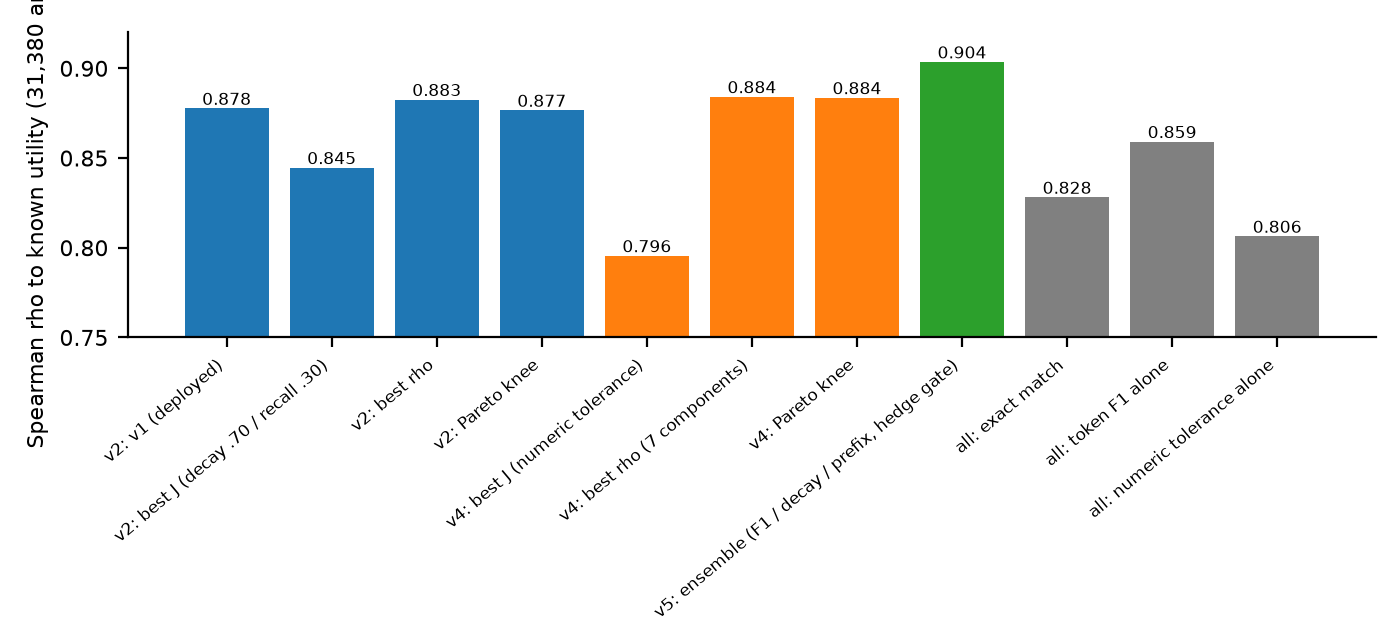
\includegraphics[width=0.85\textwidth]{fig_cmp_anchor_rho.png}\caption{Correctness of each version's scoring rule on the same 31,380 anchors (v3 has no per-answer rule).}\label{fig:fig_cmp_anchor_rho}\end{figure}
\begin{table}[htbp]
\centering\scriptsize
\caption{Anchor correctness of each version's rule on the same 31,380 synthetic answers.}
\label{tab:cmp_anchors}
\setlength{\tabcolsep}{3pt}
\begin{tabular}{lp{0.700\linewidth}rrr}
\toprule
version & rule & rho & auc & wrong mean \\
\midrule
v2 & v1 (deployed) & 0.878 & 0.994 & 0.034 \\
v2 & best J (decay .70 / recall .30) & 0.845 & 0.994 & 0.037 \\
v2 & best rho & 0.883 & 0.994 & 0.034 \\
v2 & Pareto knee & 0.877 & 0.994 & 0.036 \\
v4 & best J (numeric tolerance) & 0.796 & 0.989 & 0.022 \\
v4 & best rho (7 components) & 0.884 & 0.994 & 0.053 \\
v4 & Pareto knee & 0.884 & 0.994 & 0.039 \\
v5 & ensemble (F1 / decay / prefix, hedge gate) & 0.904 & 0.996 & 0.032 \\
all & exact match & 0.828 & 0.989 & 0.011 \\
all & token F1 alone & 0.859 & 0.965 & 0.032 \\
all & numeric tolerance alone & 0.806 & 0.919 & 0.016 \\
\bottomrule
\end{tabular}
\end{table}



\subsection{Which search finds something real}
Under the agreement objective (v2, v4) the in-sample winner loses about 0.05 when held out and ends within noise of v1 (-0.008 for v2, -0.002 for v4); the plateau covers almost every candidate in both. v3's split-half test gives the same picture for the choice of pooling rule: the selected mix beats pure Bradley--Terry by +0.024 with an interval through zero, and the uniform mix does as well. v5 is the only version whose selection survives its honesty test: the same three metrics are chosen in 90\,\% of leave-one-dataset-out folds, held-out $\rho$ moves by 0.001, and the result is +0.080 above the native typed metric on the same folds (Figure~\ref{fig:fig_cmp_honesty}, Table~\ref{tab:cmp_honesty}). The reason is the objective, not the search: agreement among the ranked models is flat over the weight space, correctness against an external signal is not.
\begin{figure}[htbp]\centering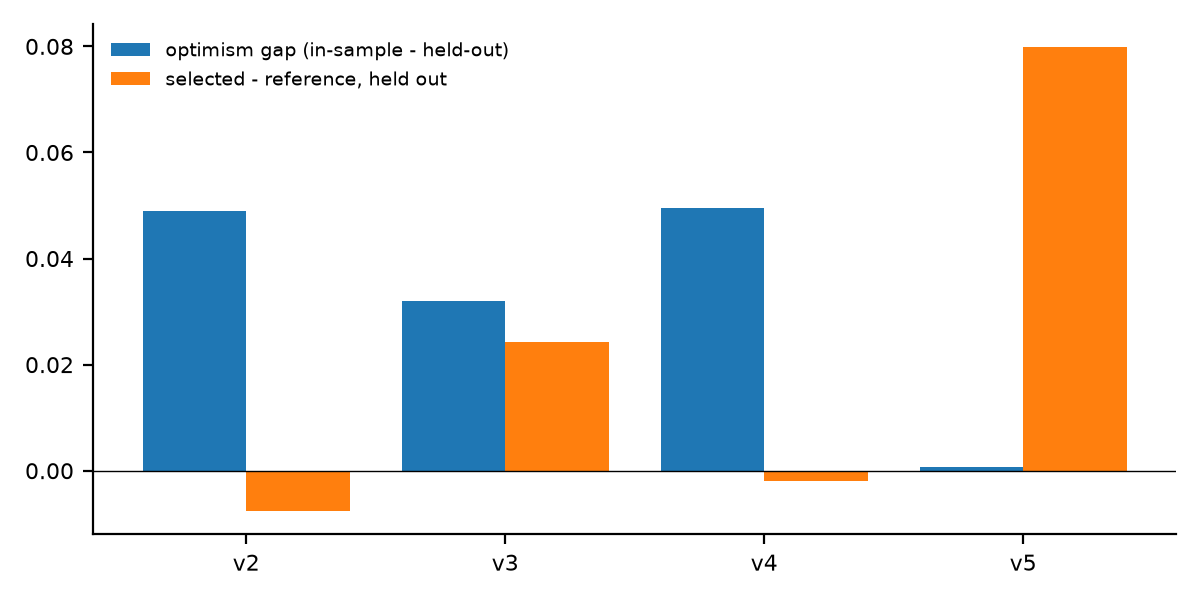
\includegraphics[width=0.7\textwidth]{fig_cmp_honesty.png}\caption{Honest-selection outcome per version: how much the in-sample winner loses when held out, and whether it still beats the version's reference rule.}\label{fig:fig_cmp_honesty}\end{figure}
\begin{table}[htbp]
\centering\tiny
\caption{Honest-selection outcome per version.}
\label{tab:cmp_honesty}
\setlength{\tabcolsep}{3pt}
\begin{tabular}{lp{0.295\linewidth}p{0.062\linewidth}p{0.160\linewidth}p{0.098\linewidth}p{0.124\linewidth}p{0.083\linewidth}}
\toprule
version & test & optimism gap & selected - reference (held out) & reference & distinct selections & plateau \\
\midrule
v2 & nested item bootstrap (B = 1,000) & 0.049 & -0.008 & v1 weights & 608 & 1765 of 1,771 \\
v3 & split-half (20 splits) & 0.032 & 0.024 & pure Bradley-Terry & 10 & -- \\
v4 & nested item bootstrap (B = 1,000) & 0.050 & -0.002 & v1 rubric & 204 & 305 of 305 \\
v5 & leave-one-dataset-out re-selection + utility perturbation & 0.001 & 0.080 & native typed metric & same set in 90\% of folds & top-100 ensemble \\
\bottomrule
\end{tabular}
\end{table}



\subsection{Transfer and designs}
Re-fitted weights predict a held-out dataset no better than v1 in v2 or v4 (Figure~\ref{fig:fig_cmp_transfer}). Sampled designs find the optimum whenever it exists (regret $\le$ 0.005 in v2, $\le$ 0.0015 in v5); in v4's nine-dimensional space the uniform lattice has the best coverage and the best found value, and the three designs agree to 0.01 (Figure~\ref{fig:fig_cmp_designs}).
\begin{figure}[htbp]\centering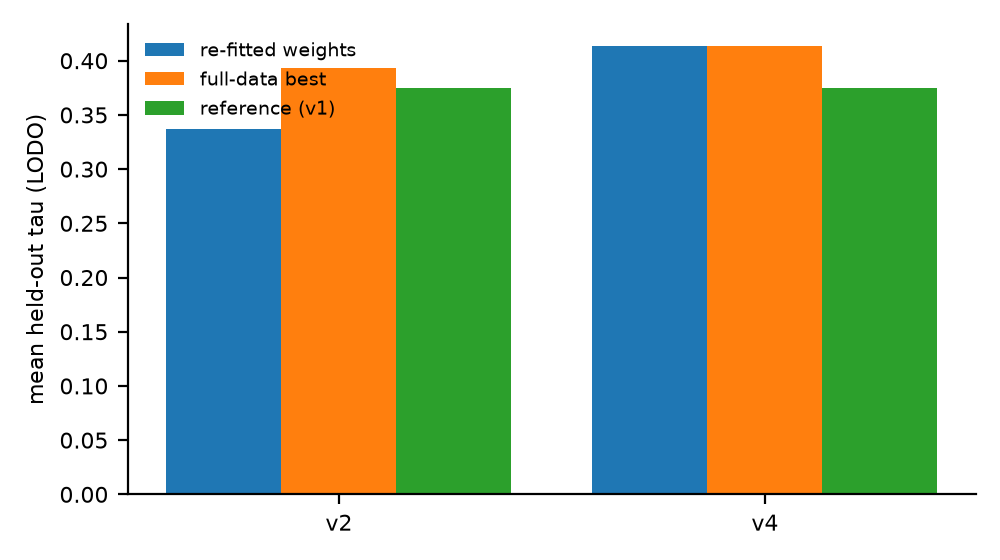
\includegraphics[width=0.6\textwidth]{fig_cmp_transfer.png}\caption{Leave-one-dataset-out transfer for the two versions that search per-answer weights under the agreement objective.}\label{fig:fig_cmp_transfer}\end{figure}
\begin{figure}[htbp]\centering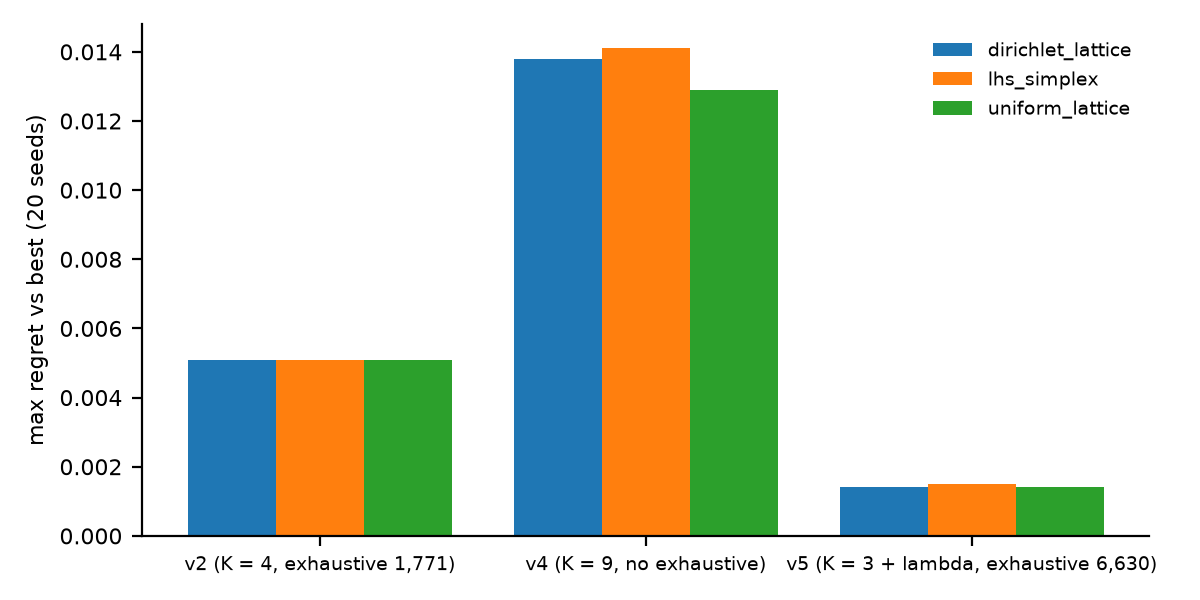
\includegraphics[width=0.7\textwidth]{fig_cmp_designs.png}\caption{Sampled-design regret per version: with few weights every design finds the optimum; with nine the lattice design is marginally better.}\label{fig:fig_cmp_designs}\end{figure}


\subsection{The leaderboard every version produces}
The same answers give the same ends under every rule and every version: Llama 3.3 70B last, gpt-oss-120b ninth, and {Claude Opus 5, GPT-5.5, Gemini 3.8 Flash} as the top three, with Friedman $p < 0.001$ and Holm-significant separation of the top group from the bottom two (Table~\ref{tab:cmp_significance}). What changes is the order inside the top three (Figure~\ref{fig:fig_cmp_ranks}): exact match and v4's numeric-tolerance rule put Opus first; the graded rules (v1, v2 best, v4 best-$\rho$, v5 ensemble) put Gemini 3.8 Flash first by Bradley--Terry and GPT-5.5 or Opus first by Borda; v3's native-metric pooling puts Gemini Flash first by Bradley--Terry and GPT-5.5 by Borda. Kendall's $W$ among datasets is 0.25--0.28 everywhere: the datasets disagree about the middle of the table regardless of rule.
\begin{figure}[htbp]\centering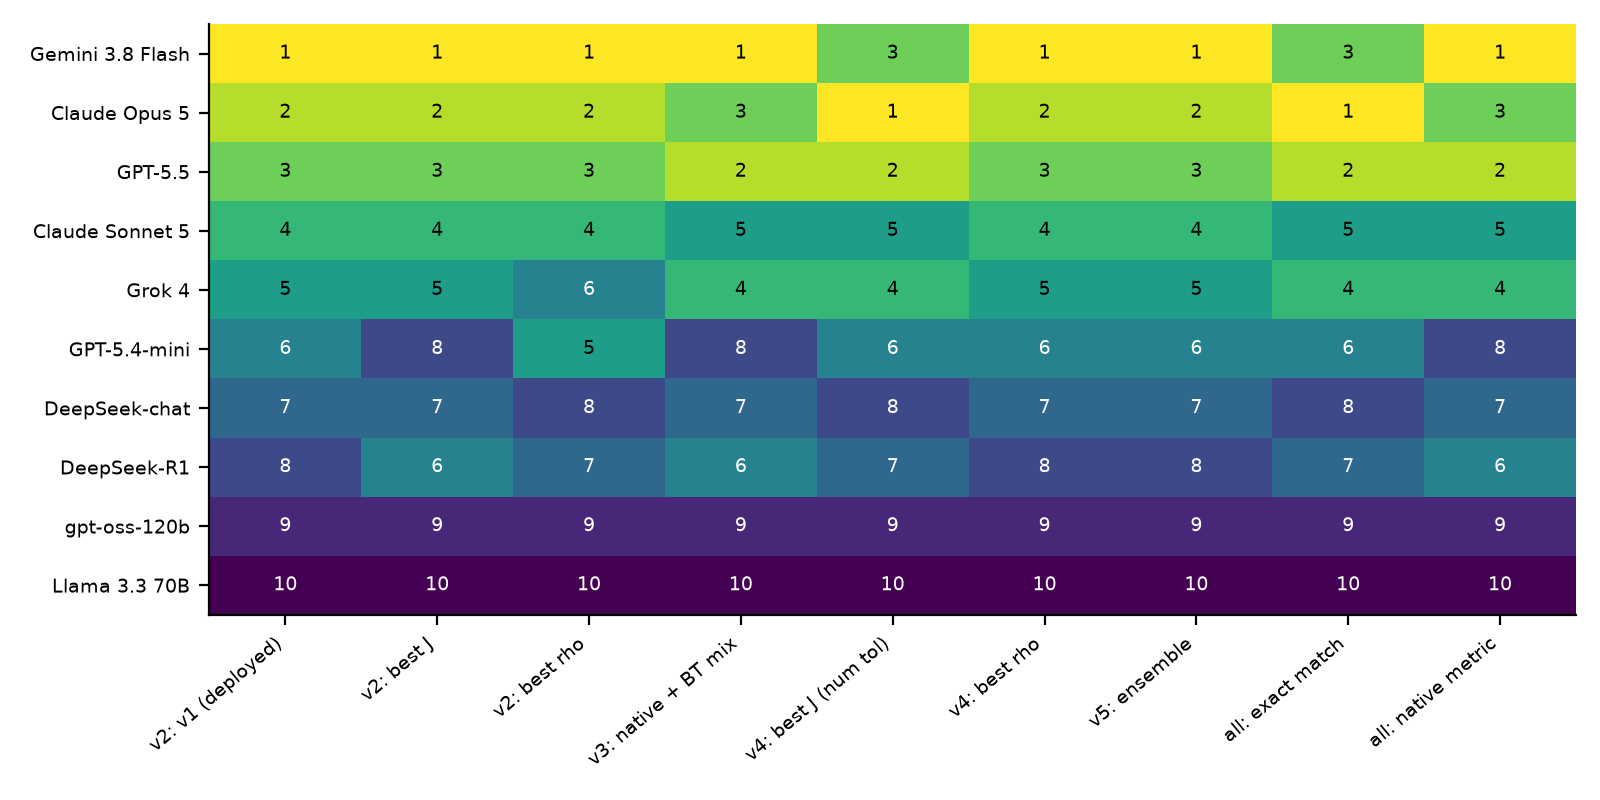
\includegraphics[width=0.85\textwidth]{fig_cmp_ranks.png}\caption{Bradley--Terry rank of every model under each version's headline rule(s) and the two common baselines.}\label{fig:fig_cmp_ranks}\end{figure}
\begin{table}[htbp]
\centering\tiny
\caption{Leaderboard significance per headline rule.}
\label{tab:cmp_significance}
\setlength{\tabcolsep}{3pt}
\begin{tabular}{lp{0.142\linewidth}rrp{0.195\linewidth}p{0.142\linewidth}p{0.115\linewidth}p{0.115\linewidth}}
\toprule
version & rule & Kendall W & Friedman p & Holm-significant pairs & first (BT) & first (Borda) & last \\
\midrule
v2 & v1 (deployed) & 0.264 & 0.000 & 13 & Gemini 3.8 Flash & GPT-5.5 & Llama 3.3 70B \\
v2 & best J & 0.264 & 0.000 & 12 & Gemini 3.8 Flash & Claude Opus 5 & Llama 3.3 70B \\
v2 & best rho & 0.256 & 0.000 & 12 & Gemini 3.8 Flash & GPT-5.5 & Llama 3.3 70B \\
v3 & native + BT mix & 0.274 & 0.000 & 13 & Gemini 3.8 Flash & GPT-5.5 & Llama 3.3 70B \\
v4 & best J (num tol) & 0.276 & 0.000 & 13 & Claude Opus 5 & Claude Opus 5 & Llama 3.3 70B \\
v4 & best rho & 0.272 & 0.000 & 12 & Gemini 3.8 Flash & GPT-5.5 & Llama 3.3 70B \\
v5 & ensemble & 0.259 & 0.000 & 11 & Gemini 3.8 Flash & Claude Opus 5 & Llama 3.3 70B \\
all & exact match & 0.279 & 0.000 & 12 & Claude Opus 5 & Claude Opus 5 & Llama 3.3 70B \\
all & native metric & 0.283 & 0.000 & 13 & Gemini 3.8 Flash & GPT-5.5 & Llama 3.3 70B \\
\bottomrule
\end{tabular}
\end{table}

\begin{figure}[htbp]\centering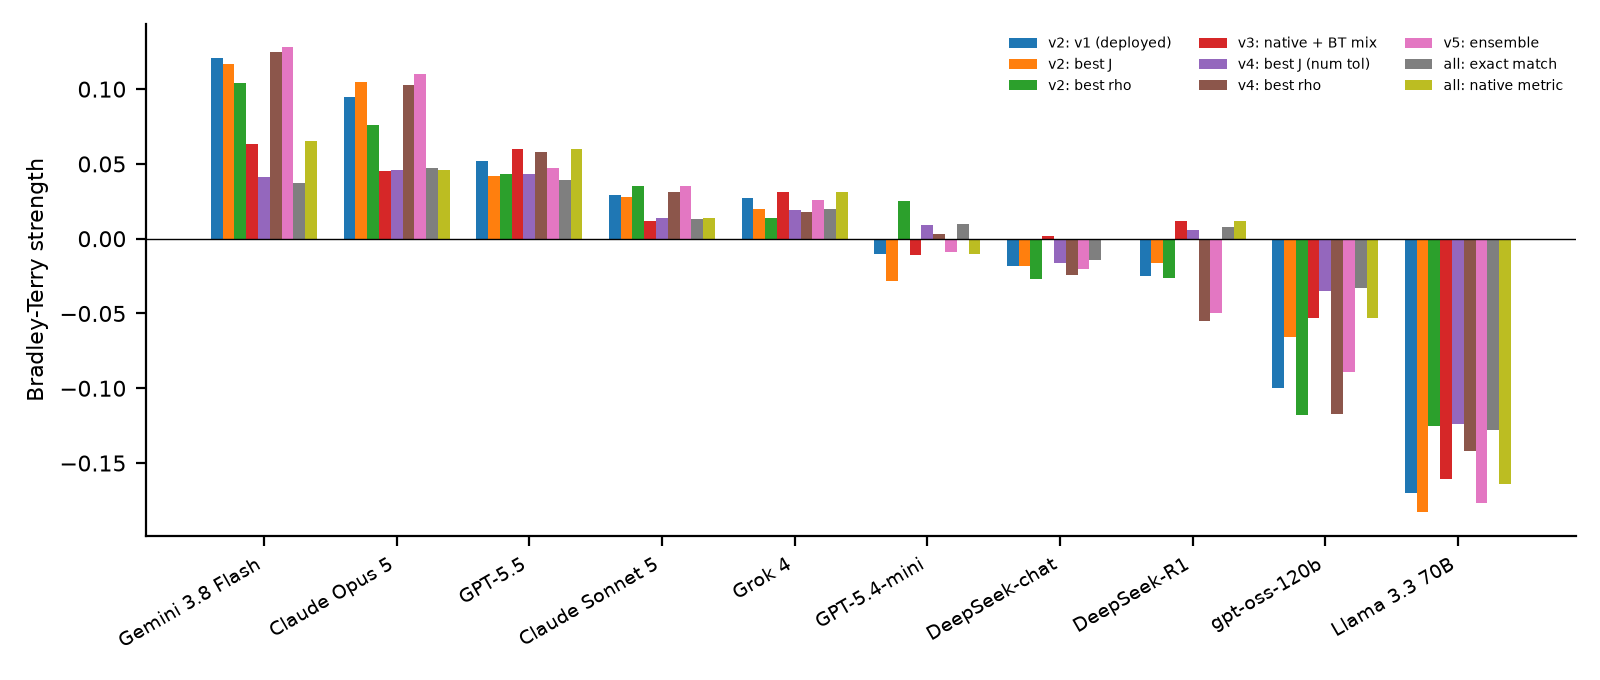
\includegraphics[width=0.85\textwidth]{fig_cmp_bt.png}\caption{Bradley--Terry strengths per model under each version's headline rule(s).}\label{fig:fig_cmp_bt}\end{figure}
\begin{figure}[htbp]\centering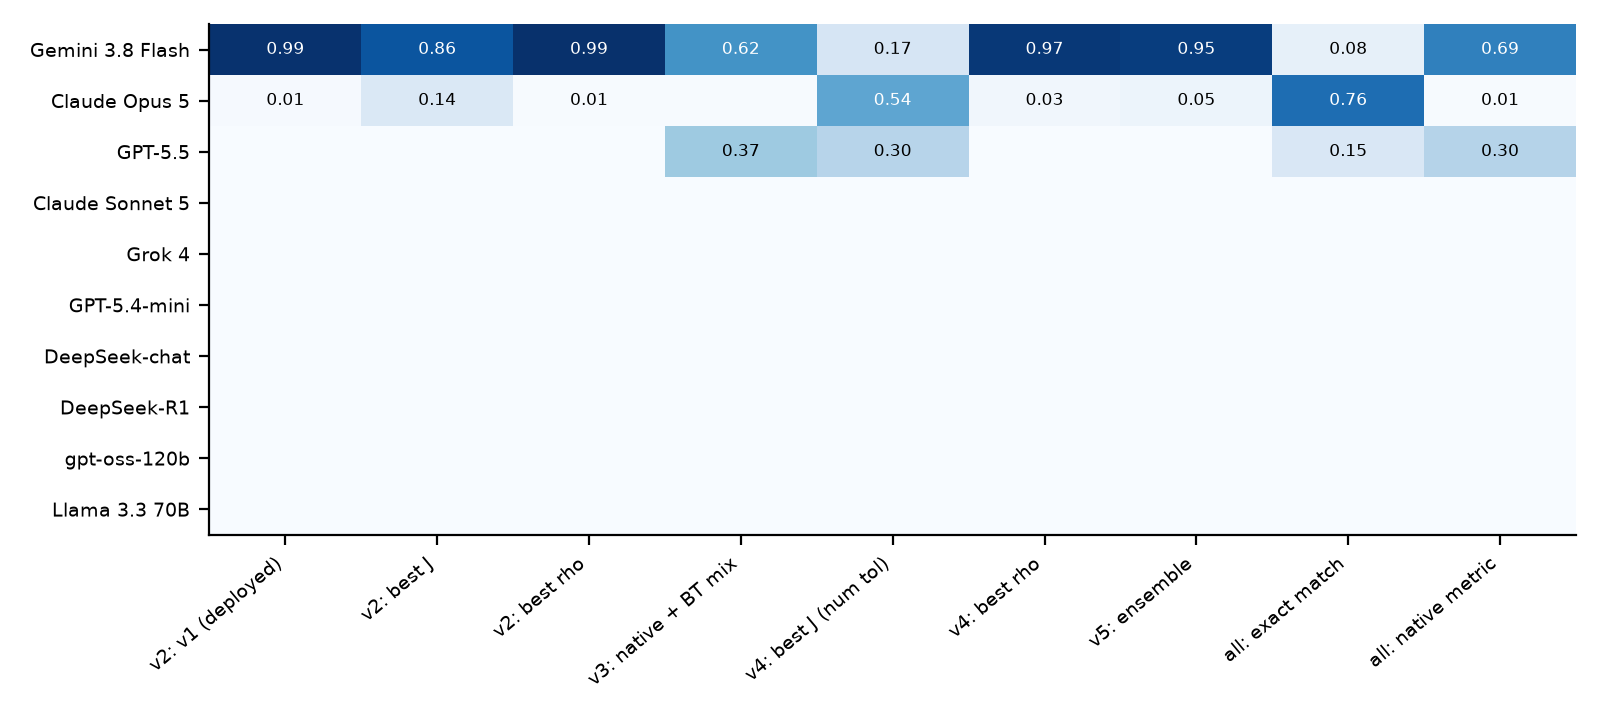
\includegraphics[width=0.85\textwidth]{fig_cmp_p_first.png}\caption{Bootstrap probability of first place under each headline rule.}\label{fig:fig_cmp_p_first}\end{figure}


\section{What is better, per version}
\begin{description}[style=unboxed,leftmargin=0pt]
\item[] \textbf{v2 (exhaustive grid over v1's weights).} Best at answering the question it was built for: it proves, not samples, that no weighting of v1's ingredients is distinguishable from v1 on this suite (plateau 1,765 of 1,771; out-of-bag difference $-0.008$ with an interval through zero). It is the right headline for ``the deployed weights are fine''. It cannot say the weights are \emph{right}, because agreement is not correctness.
\item[] \textbf{v3 (aggregation views).} Best at the pooling question and the only version that reports fitted parameters with standard errors (Bradley--Terry, Rasch, Kemeny cost). Its finding is that mixing views buys little over the uniform mix and that pure Bradley--Terry is the least reproducible single rule on 31 datasets $\times$ 10 models. It has no per-answer rule, so it cannot audit the judge's formula.
\item[] \textbf{v4 (nine components).} Best as the negative control: adding five components and sampling 305 candidates in a 3-million-point space finds that a single typed metric (numeric tolerance) maximises agreement, and that this metric is the worst on correctness. It shows most clearly that the agreement objective rewards coarseness. Its search cannot be exhaustive, so its optimum is only ``best found''.
\item[] \textbf{v5 (anchor-calibrated ensemble).} Best scoring rule by the external signal ($\rho$ 0.904, AUC 0.996) and the only selection that survives leave-one-dataset-out unchanged. It is the version to deploy if the goal is to score answers well; its weakness is that the signal is synthetic (a hand-set utility scale) until human labels exist, and its gain over v1 (+0.026 in $\rho$) is real but small.
\item[] \textbf{Taken together.} v2 and v4 establish that the weight question has no answer on this suite; v3 establishes that the pooling question has no strong answer either; v5 establishes that the correctness question does, and that the deployed rule is close to its answer. The paper's claim is therefore: keep v1 (or the v5 ensemble), report the leaderboard under several rules with the ends and the significant pairs, and spend the next effort on human labels rather than on more weight search.
\end{description}

\clearpage
\appendix
\section{All figures}
Every figure that can be drawn from the saved outputs; source data in \texttt{data/}.
\begin{figure}[htbp]\centering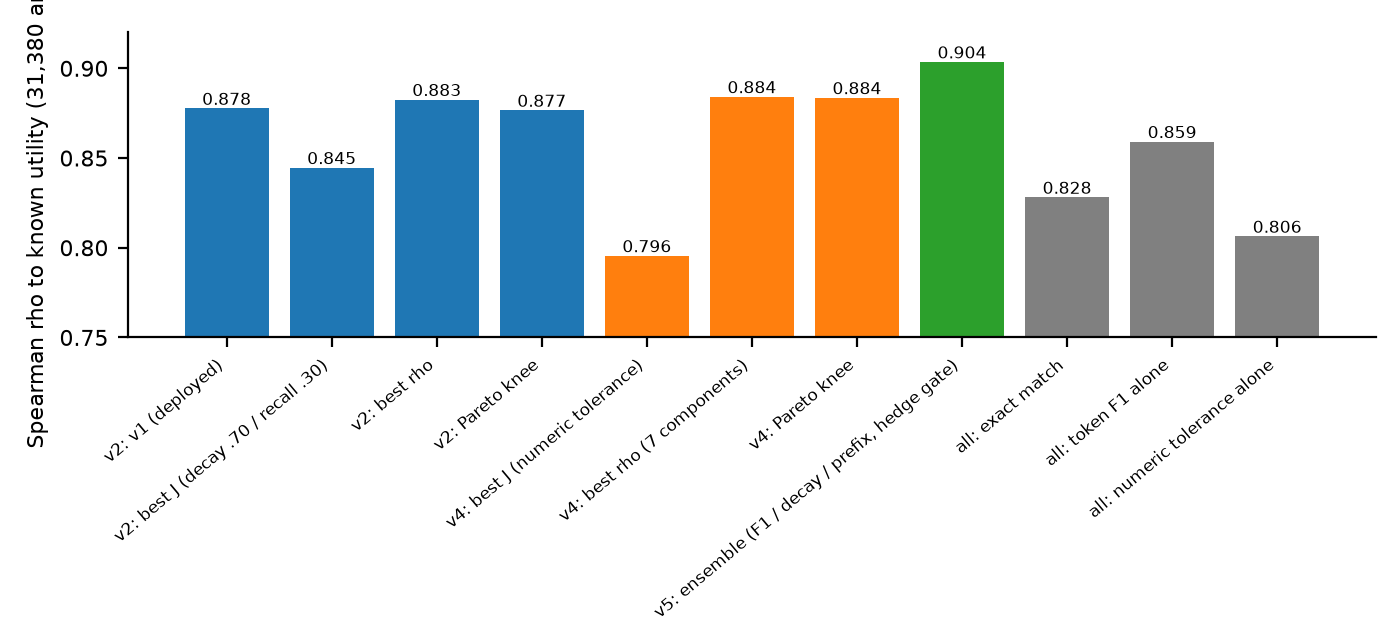
\includegraphics[width=0.9\textwidth]{fig_cmp_anchor_rho.png}\caption{Correctness of each version's scoring rule on the same 31,380 anchors (v3 has no per-answer rule).}\label{figall:fig_cmp_anchor_rho}\end{figure}
\begin{figure}[htbp]\centering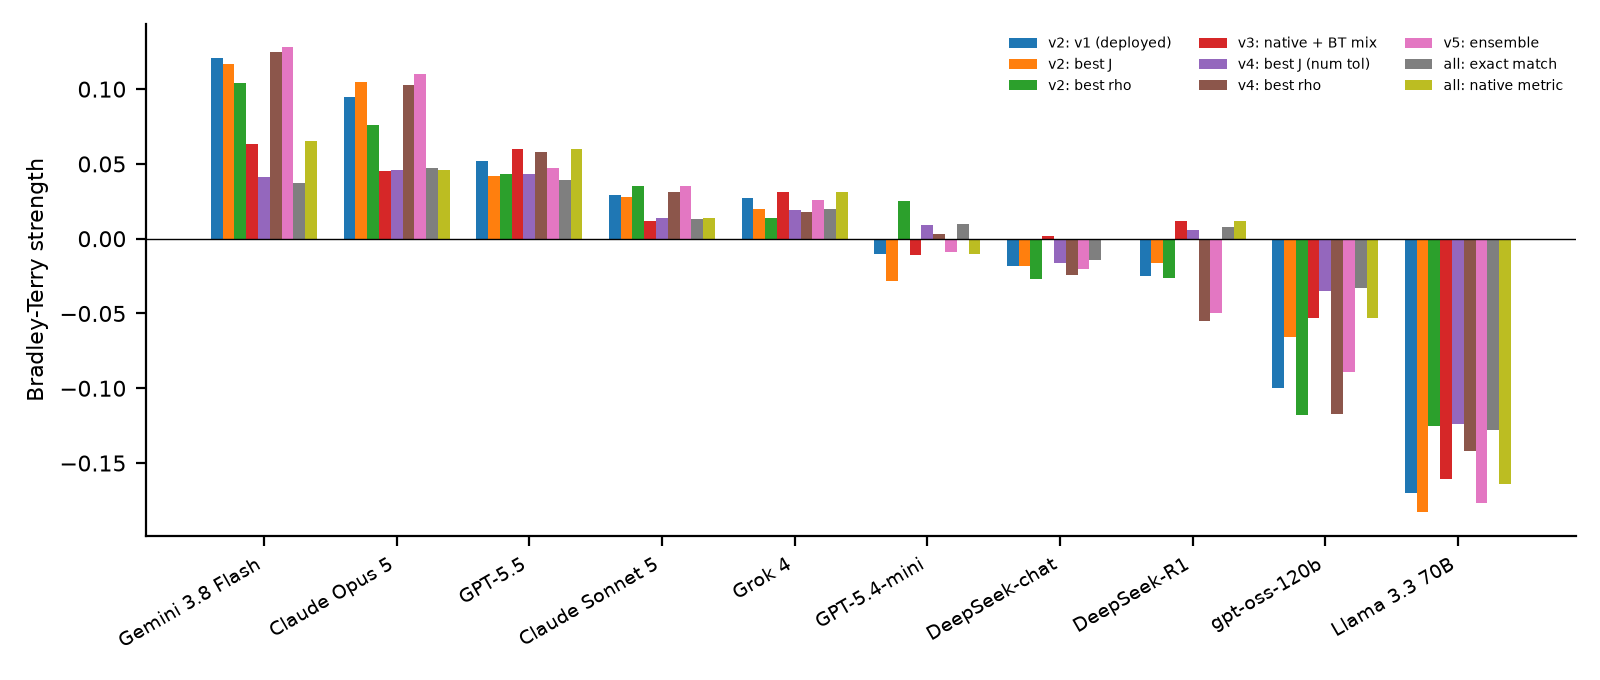
\includegraphics[width=0.9\textwidth]{fig_cmp_bt.png}\caption{Bradley--Terry strengths per model under each version's headline rule(s).}\label{figall:fig_cmp_bt}\end{figure}
\begin{figure}[htbp]\centering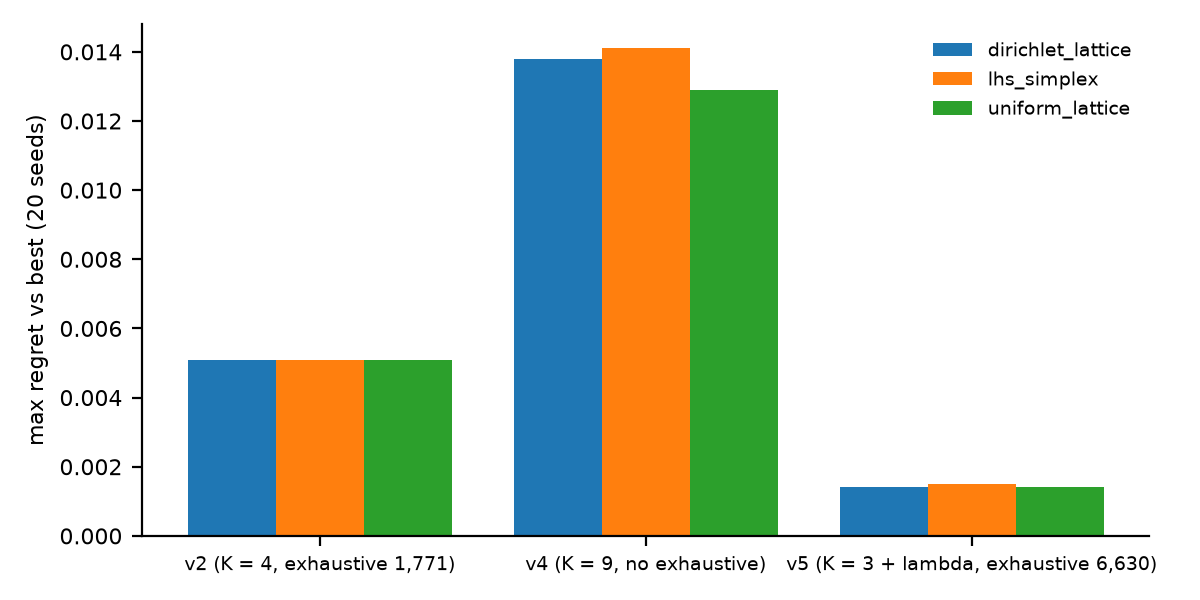
\includegraphics[width=0.9\textwidth]{fig_cmp_designs.png}\caption{Sampled-design regret per version: with few weights every design finds the optimum; with nine the lattice design is marginally better.}\label{figall:fig_cmp_designs}\end{figure}
\begin{figure}[htbp]\centering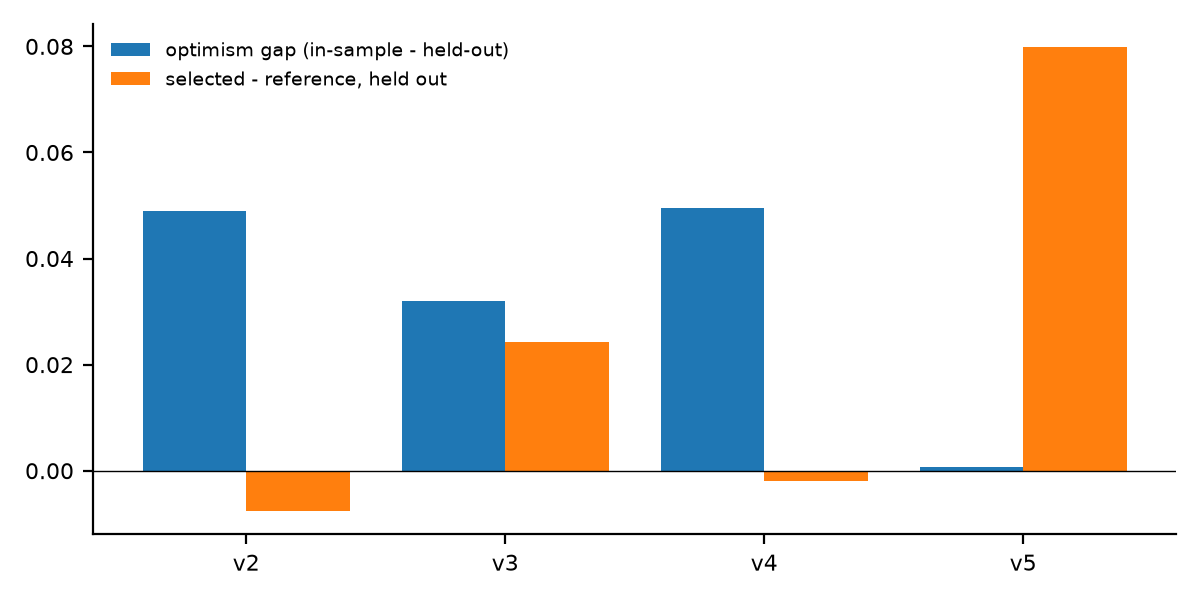
\includegraphics[width=0.9\textwidth]{fig_cmp_honesty.png}\caption{Honest-selection outcome per version: how much the in-sample winner loses when held out, and whether it still beats the version's reference rule.}\label{figall:fig_cmp_honesty}\end{figure}
\begin{figure}[htbp]\centering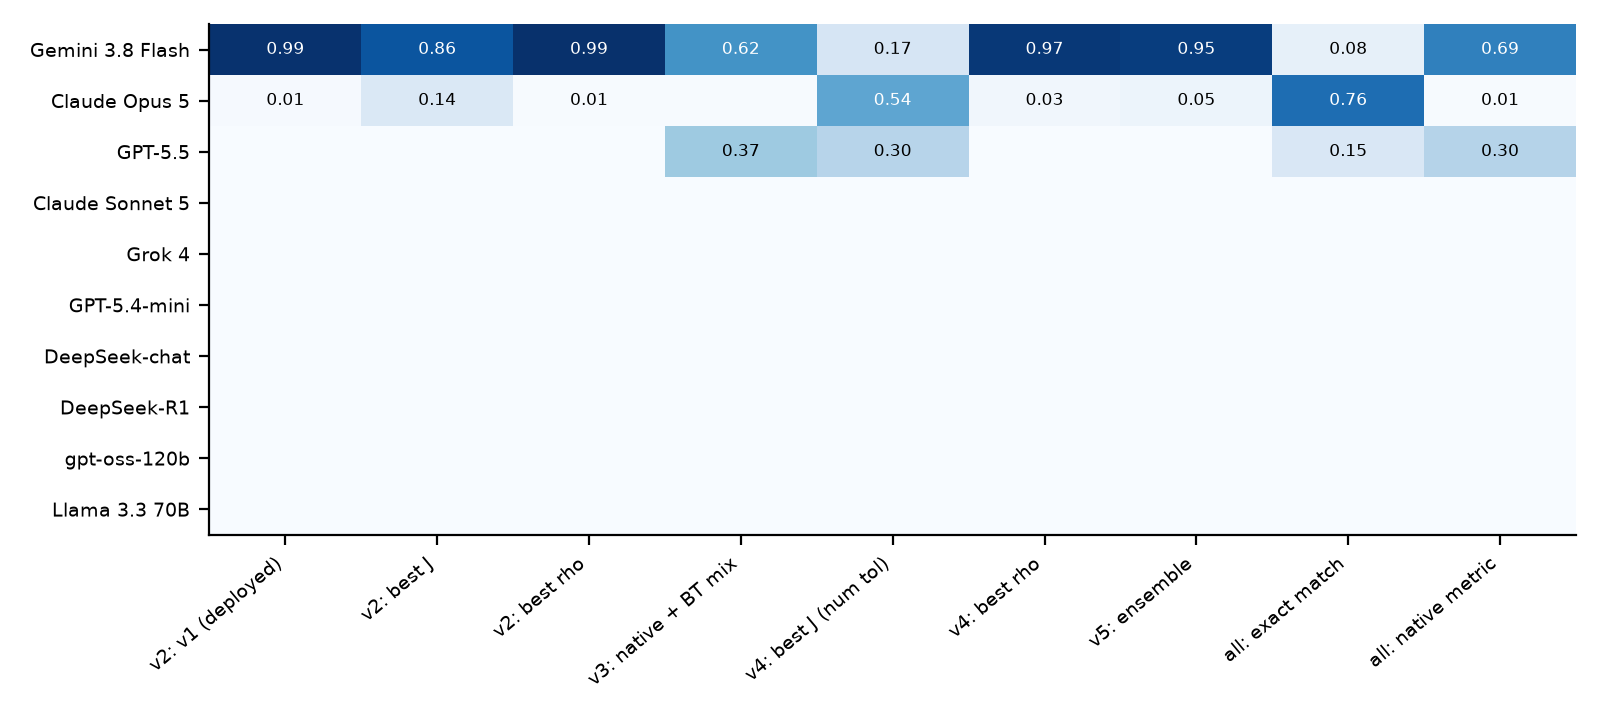
\includegraphics[width=0.9\textwidth]{fig_cmp_p_first.png}\caption{Bootstrap probability of first place under each headline rule.}\label{figall:fig_cmp_p_first}\end{figure}
\begin{figure}[htbp]\centering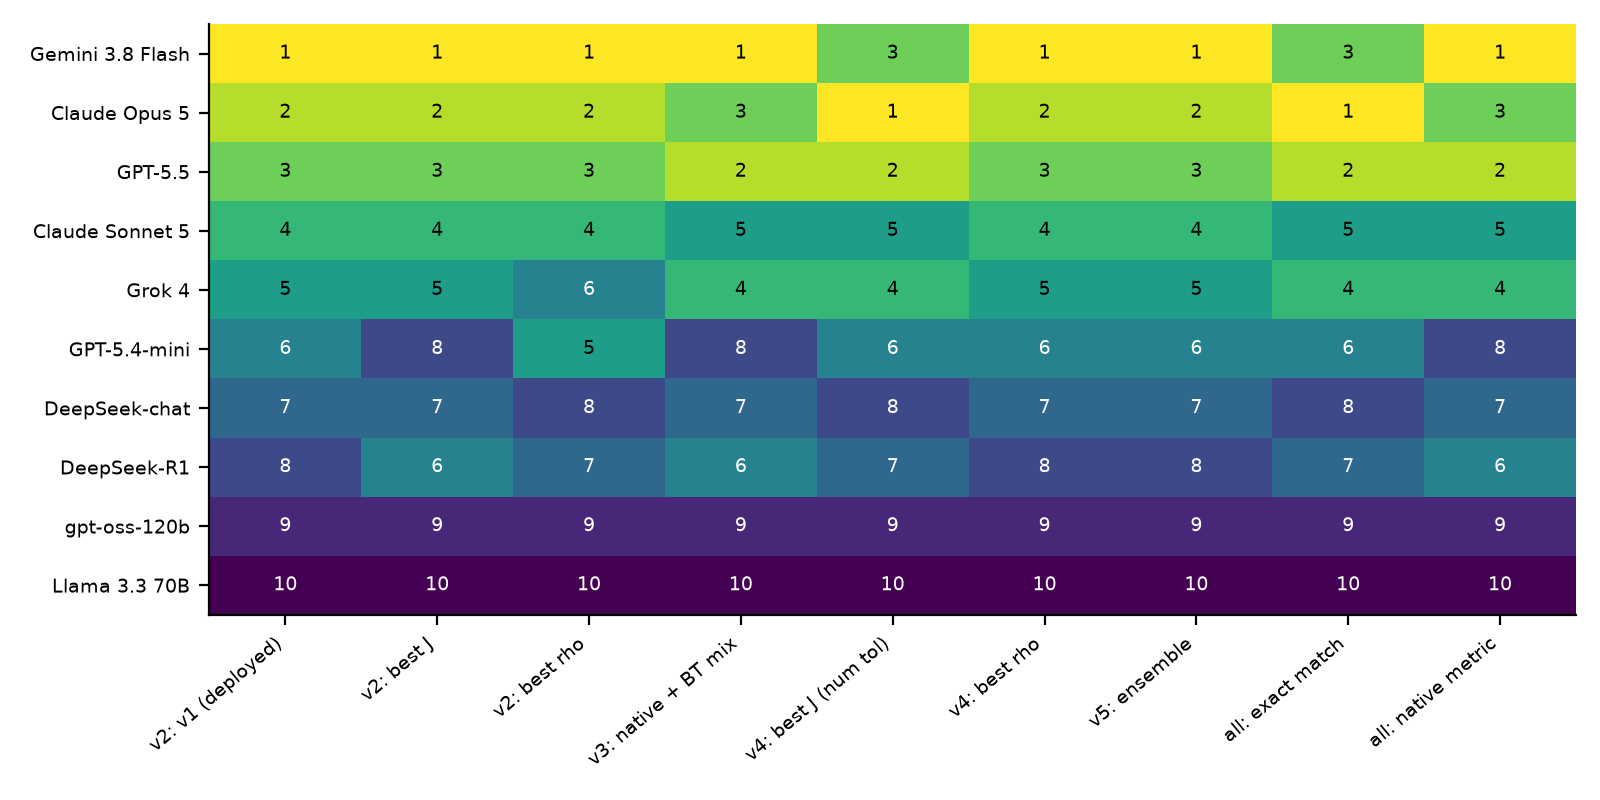
\includegraphics[width=0.9\textwidth]{fig_cmp_ranks.png}\caption{Bradley--Terry rank of every model under each version's headline rule(s) and the two common baselines.}\label{figall:fig_cmp_ranks}\end{figure}
\begin{figure}[htbp]\centering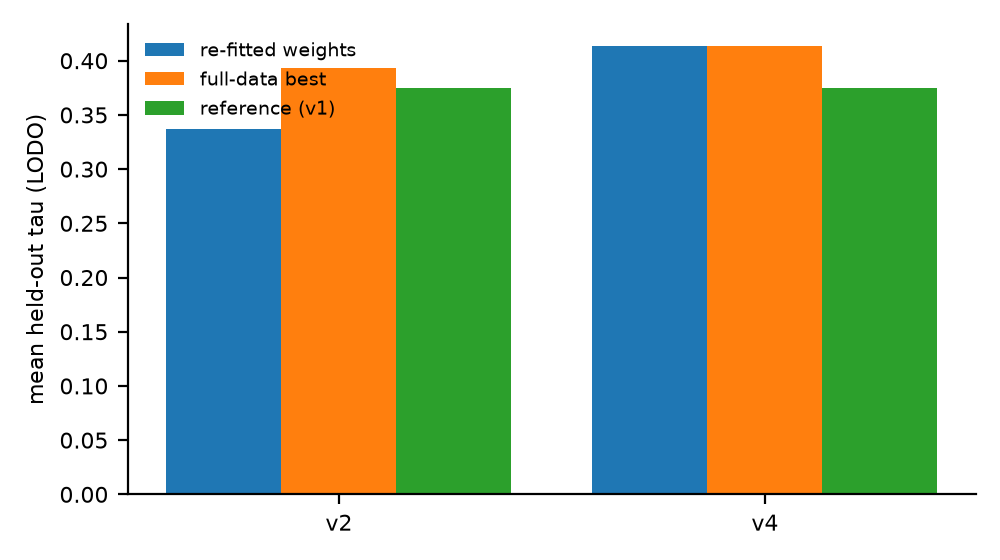
\includegraphics[width=0.9\textwidth]{fig_cmp_transfer.png}\caption{Leave-one-dataset-out transfer for the two versions that search per-answer weights under the agreement objective.}\label{figall:fig_cmp_transfer}\end{figure}
\clearpage
\section{All tables}
Every saved table, one file each under \texttt{tables/}; include any in the main text with \texttt{\textbackslash input}.
\begin{table}[htbp]
\centering\scriptsize
\caption{Anchor correctness of each version's rule on the same 31,380 synthetic answers.}
\label{tab:cmp_anchors}
\setlength{\tabcolsep}{3pt}
\begin{tabular}{lp{0.700\linewidth}rrr}
\toprule
version & rule & rho & auc & wrong mean \\
\midrule
v2 & v1 (deployed) & 0.878 & 0.994 & 0.034 \\
v2 & best J (decay .70 / recall .30) & 0.845 & 0.994 & 0.037 \\
v2 & best rho & 0.883 & 0.994 & 0.034 \\
v2 & Pareto knee & 0.877 & 0.994 & 0.036 \\
v4 & best J (numeric tolerance) & 0.796 & 0.989 & 0.022 \\
v4 & best rho (7 components) & 0.884 & 0.994 & 0.053 \\
v4 & Pareto knee & 0.884 & 0.994 & 0.039 \\
v5 & ensemble (F1 / decay / prefix, hedge gate) & 0.904 & 0.996 & 0.032 \\
all & exact match & 0.828 & 0.989 & 0.011 \\
all & token F1 alone & 0.859 & 0.965 & 0.032 \\
all & numeric tolerance alone & 0.806 & 0.919 & 0.016 \\
\bottomrule
\end{tabular}
\end{table}

\clearpage
\begin{table}[htbp]
\centering\scriptsize
\caption{What each version does.}
\label{tab:cmp_design}
\setlength{\tabcolsep}{3pt}
\begin{tabular}{p{0.103\linewidth}p{0.186\linewidth}p{0.178\linewidth}p{0.169\linewidth}p{0.264\linewidth}}
\toprule
 & v2 & v3 & v4 & v5 \\
\midrule
per-answer rule & 4 metrics (F1, decay, P, R), weights searched & dataset's own metric & 9 metrics, weights searched & 3 of 100 metrics, weights searched, top-100 ensemble, hedge gate \\
what is searched & 4 weights, exhaustive (1,771) & mix of 8 aggregation views (455 candidates) & 9 weights, 3 sampled designs (305) & 3 weights + lambda, exhaustive (6,630) \\
objective & datasets agree (tau to Borda pool) & stability + transitivity + consensus & datasets agree (tau to Borda pool) & anchor rho, AUC, JS consistency, native tau, wrong -> 0 \\
checked against & the ranked models (+ anchors beside) & bootstrap resamples & the ranked models (+ anchors beside) & 31,380 synthetic answers of known quality \\
honesty test & nested item bootstrap, plateau, LODO/LOFO & split-half vs pure BT / uniform & nested item bootstrap, plateau, LODO/LOFO & LODO re-selection, utility perturbation, probes \\
headline leaderboard rule & v1 weights (deployed) & native metric, Bradley-Terry & v1 rubric (comparability) & calibrated ensemble \\
main risk & circular: agreement is not correctness & views differ in kind; no per-answer rule & circular; 9-D space not enumerable & hand-set utility scale; synthetic anchors \\
\bottomrule
\end{tabular}
\end{table}

\clearpage
\begin{table}[htbp]
\centering\scriptsize
\caption{Sampled-design regret per version.}
\label{tab:cmp_designs}
\setlength{\tabcolsep}{3pt}
\begin{tabular}{p{0.492\linewidth}p{0.226\linewidth}p{0.146\linewidth}r}
\toprule
version & design & regret mean & regret max \\
\midrule
v2 (K = 4, exhaustive 1,771) & dirichlet\_\allowbreak{}lattice & 0.0038 & 0.0051 \\
v2 (K = 4, exhaustive 1,771) & lhs\_\allowbreak{}simplex & 0.0034 & 0.0051 \\
v2 (K = 4, exhaustive 1,771) & uniform\_\allowbreak{}lattice & 0.0029 & 0.0051 \\
v4 (K = 9, no exhaustive) & dirichlet\_\allowbreak{}lattice & 0.0100 & 0.0138 \\
v4 (K = 9, no exhaustive) & lhs\_\allowbreak{}simplex & 0.0107 & 0.0141 \\
v4 (K = 9, no exhaustive) & uniform\_\allowbreak{}lattice & 0.0077 & 0.0129 \\
v5 (K = 3 + lambda, exhaustive 6,630) & dirichlet\_\allowbreak{}lattice & 0.0007 & 0.0014 \\
v5 (K = 3 + lambda, exhaustive 6,630) & lhs\_\allowbreak{}simplex & 0.0008 & 0.0015 \\
v5 (K = 3 + lambda, exhaustive 6,630) & uniform\_\allowbreak{}lattice & 0.0007 & 0.0014 \\
\bottomrule
\end{tabular}
\end{table}

\clearpage
\begin{table}[htbp]
\centering\tiny
\caption{Honest-selection outcome per version.}
\label{tab:cmp_honesty}
\setlength{\tabcolsep}{3pt}
\begin{tabular}{lp{0.295\linewidth}p{0.062\linewidth}p{0.160\linewidth}p{0.098\linewidth}p{0.124\linewidth}p{0.083\linewidth}}
\toprule
version & test & optimism gap & selected - reference (held out) & reference & distinct selections & plateau \\
\midrule
v2 & nested item bootstrap (B = 1,000) & 0.049 & -0.008 & v1 weights & 608 & 1765 of 1,771 \\
v3 & split-half (20 splits) & 0.032 & 0.024 & pure Bradley-Terry & 10 & -- \\
v4 & nested item bootstrap (B = 1,000) & 0.050 & -0.002 & v1 rubric & 204 & 305 of 305 \\
v5 & leave-one-dataset-out re-selection + utility perturbation & 0.001 & 0.080 & native typed metric & same set in 90\% of folds & top-100 ensemble \\
\bottomrule
\end{tabular}
\end{table}

\clearpage
\begin{landscape}
\begin{table}[htbp]
\centering\tiny
\caption{Bradley--Terry rank per model under each headline rule.}
\label{tab:cmp_ranks}
\setlength{\tabcolsep}{3pt}
\resizebox{\linewidth}{!}{%
\begin{tabular}{lrrrrrrrrr}
\toprule
model & v2: v1 (deployed) & v2: best J & v2: best rho & v3: native + BT mix & v4: best J (num tol) & v4: best rho & v5: ensemble & all: exact match & all: native metric \\
\midrule
Gemini 3.8 Flash & 1 & 1 & 1 & 1 & 3 & 1 & 1 & 3 & 1 \\
Claude Opus 5 & 2 & 2 & 2 & 3 & 1 & 2 & 2 & 1 & 3 \\
GPT-5.5 & 3 & 3 & 3 & 2 & 2 & 3 & 3 & 2 & 2 \\
Claude Sonnet 5 & 4 & 4 & 4 & 5 & 5 & 4 & 4 & 5 & 5 \\
Grok 4 & 5 & 5 & 6 & 4 & 4 & 5 & 5 & 4 & 4 \\
GPT-5.4-mini & 6 & 8 & 5 & 8 & 6 & 6 & 6 & 6 & 8 \\
DeepSeek-chat & 7 & 7 & 8 & 7 & 8 & 7 & 7 & 8 & 7 \\
DeepSeek-R1 & 8 & 6 & 7 & 6 & 7 & 8 & 8 & 7 & 6 \\
gpt-oss-120b & 9 & 9 & 9 & 9 & 9 & 9 & 9 & 9 & 9 \\
Llama 3.3 70B & 10 & 10 & 10 & 10 & 10 & 10 & 10 & 10 & 10 \\
\bottomrule
\end{tabular}
}
\end{table}
\end{landscape}

\clearpage
\begin{table}[htbp]
\centering\tiny
\caption{Leaderboard significance per headline rule.}
\label{tab:cmp_significance}
\setlength{\tabcolsep}{3pt}
\begin{tabular}{lp{0.142\linewidth}rrp{0.195\linewidth}p{0.142\linewidth}p{0.115\linewidth}p{0.115\linewidth}}
\toprule
version & rule & Kendall W & Friedman p & Holm-significant pairs & first (BT) & first (Borda) & last \\
\midrule
v2 & v1 (deployed) & 0.264 & 0.000 & 13 & Gemini 3.8 Flash & GPT-5.5 & Llama 3.3 70B \\
v2 & best J & 0.264 & 0.000 & 12 & Gemini 3.8 Flash & Claude Opus 5 & Llama 3.3 70B \\
v2 & best rho & 0.256 & 0.000 & 12 & Gemini 3.8 Flash & GPT-5.5 & Llama 3.3 70B \\
v3 & native + BT mix & 0.274 & 0.000 & 13 & Gemini 3.8 Flash & GPT-5.5 & Llama 3.3 70B \\
v4 & best J (num tol) & 0.276 & 0.000 & 13 & Claude Opus 5 & Claude Opus 5 & Llama 3.3 70B \\
v4 & best rho & 0.272 & 0.000 & 12 & Gemini 3.8 Flash & GPT-5.5 & Llama 3.3 70B \\
v5 & ensemble & 0.259 & 0.000 & 11 & Gemini 3.8 Flash & Claude Opus 5 & Llama 3.3 70B \\
all & exact match & 0.279 & 0.000 & 12 & Claude Opus 5 & Claude Opus 5 & Llama 3.3 70B \\
all & native metric & 0.283 & 0.000 & 13 & Gemini 3.8 Flash & GPT-5.5 & Llama 3.3 70B \\
\bottomrule
\end{tabular}
\end{table}

\clearpage
\begin{table}[htbp]
\centering\scriptsize
\caption{Leave-one-dataset-out transfer (mean held-out $\tau$).}
\label{tab:cmp_transfer}
\setlength{\tabcolsep}{3pt}
\begin{tabular}{lp{0.326\linewidth}p{0.269\linewidth}p{0.269\linewidth}}
\toprule
version & re-fitted weights & full-data best & reference (v1) \\
\midrule
v2 & 0.337 & 0.393 & 0.374 \\
v4 & 0.413 & 0.413 & 0.374 \\
\bottomrule
\end{tabular}
\end{table}

\clearpage
\end{document}
